\documentclass[a4paper,11pt]{article}

\usepackage[utf8]{inputenc}
\usepackage[italian]{babel}
\usepackage{graphicx}
\usepackage{geometry}

\newgeometry{vmargin={10mm,28mm}, hmargin={25mm,25mm}}

% Definition of \maketitle
\makeatletter
\newcommand{\departmentname}[1]{\def\@departmentname{#1}}
\newcommand{\coursename}[1]{\def\@coursename{#1}}
\newcommand{\academicyear}[1]{\def\@academicyear{#1}}
\newcommand{\advisorname}[1]{\def\@advisorname{#1}}
\newcommand{\coadvisorname}[1]{\def\@coadvisorname{#1}}
\newcommand{\studentname}[1]{\def\@studentname{#1}}
\newcommand{\itathesistitle}[1]{\def\@itathesistitle{#1}}
\newcommand{\engthesistitle}[1]{\def\@engthesistitle{#1}}

\def\@maketitle{
	\begin{center}
		
\includegraphics[width=4cm]{images/logoUnipr.png}\\[2ex]
		\@departmentname\\[1ex]
		\@coursename\\
		\noindent\rule{8cm}{0.4pt}\\[1ex]
		\@itathesistitle\\[1ex]
		\@engthesistitle
	\end{center}
	\underline{Relatore:}
	\hfill
	\underline{Tesi di Laurea di:}\\
	\@advisorname
	\hfill
	\@studentname\\[1ex]
	\underline{Correlatori:}\\
	\@coadvisorname
	\begin{center}
		\@academicyear
	\end{center}
	\vskip 0.1cm
}
\makeatother

\departmentname{\textbf{Dipartimento di Ingegneria e Architettura}}
\coursename{\textbf{Corso di Laurea in Ingegneria Informatica Elettronica e delle Telecomunicazioni}}
\academicyear{ANNO ACCADEMICO 2021/2022}
\advisorname{Prof. Michele Amoretti}
\coadvisorname{Dr Alberto Dallaporta}
\studentname{Alex Spagni}
\itathesistitle{Sviluppo di un Applicazione Mobile Multipiattaforma per la Ricerca e la Visualizzazione di Immagini}
\engthesistitle{Development of a Cross-Platform Mobile Application for Searching and Viewing Images}

\begin{document}
\maketitle
Le applicazioni mobile, ovvero applicativi che vengono eseguiti su dispositivi mobili, sono sempre pi\`u diffuse in quanto sta crescendo il numero di utenti che ne fanno uso.
Esse si distinguono in due grandi categorie: app native e app multipiattaforma; le prime sono delle applicazioni software che sono state sviluppate per funzionare su uno
specifico tipo di dispositivo o piattaforma, mentre le seconde sono applicazioni che possono essere eseguita anche su sistemi operativi differenti ma usando sempre la stessa codebase.
Per questo elaborato di Tesi \`e stata sviluppata un'applicazione multipiattaforma attraverso l'uso del framework React Native. L'app permette la ricerca di immagini scattate dai
diversi Rover inviati su Marte dalla NASA; le foto possono essere cercate in base al nome del Rover o alla data solare in cui sono state scattate. L'applicativo consente di
occultare le immagini non desiderate, in modo che non vengano mostrate in futuro; nonostante ci\`o l'utente pu\`o anche decidere di ripristinare tali immagini temporaneamente. Affinch\'e solo gli utenti
autorizzati possano usare l'applicazione, \`e stato introdotto uno strato di autenticazione tramite il quale \`e possibile registrarsi o accedere al proprio profilo.

Per poter seguire un corretto sviluppo dell'applicazione sono state effettuate diverse ricerche. Inizialmente sono stati esaminati i diversi framework che consentono lo sviluppo di applicativi multipiattaforma
e si \`e cercato uno strumento (Expo) che rendesse il suo sviluppo pi\`u rapido. Sono seguite poi diverse settimane di lettura e comprensione della documentazione ufficiale del framework per capire
come utilizzare i diversi componenti forniti. Una volta fatto ci\`o, si \`e passati alla definizione dei requisiti dell'applicazione e all' implementazione vera e propria.

Lo sviluppo dell'applicazione aveva portato diversi obiettivi, tra cui:

\begin{itemize}
    \item La possibilit\`a di poter distribuire l'applicativo su pi\`u piattaforme attraverso l'uso di un'unica code base.
    \item L'utilizzo del protocollo HTTP per la comunicazione con i server della NASA dai quali vengono prelevate le immagini, e con il server locale che assicura lo strato di autenticazione.
    \item L'utilizzo del formato JSON per la trasmissione e l'estrapolazione di dati.
    \item La gestione della navigazione tra i vari screen dell'applicazione.
    \item La comprensione e l'utilizzo dell'architettura modulare.
\end{itemize}

Tutti gli obiettivi sopra citati sono stati raggiunti con successo; in particolare, dopo aver concluso la fase di test dell'applicazione si pu\`o affermare che la visualizzazione delle immagini avviene correttamente rispettando tutti i requisiti funzionali e non funzionali.
Inoltre, la navigazione tra i vari screen che compongono l'applicazione \`e fluida e consente una buona User Experience.
Dato che l'applicazione \`e stata sviluppata secondo un'architettura modulare, \`e possibile modificare le singole parti dell'applicativo senza alterare il comportamento dell'intera applicazione; questo rappresenta un grande vantaggio in quanto permette di semplificare la fase di testing.
La grafica \`e uno degli aspetti centrali in un applicativo; grazie all'uso dello stile FlexBox l'applicazione presenta la stessa grafica su dispositivi con dimensioni e sistemi operativi diversi se non per minime differenze, come si può osservare nella Fig 1 e 2.
Tamite l'uso di React e React Native \`e stata progettata un'interfaccia per ogni stato dell'applicazione, mentre attraverso Redux ogni stato \`e mantenuto in uno store e viene modificato tramite l'uso di funzioni pure.


Nonostante l'applicazione soddisfi tutti i requisiti di progetto, si potrebbe pensare di aggiungere altre funzionalit\`a come: la possibilit\`a di ricercare le immagini in base alla camera utilizzata per scattare le foto e la possibilit\`a di ricercare le immagini per data ``Marziana".
Un altro possibile miglioramento potrebbe consistere nel memorizzare le ultime immagini visualizzate dall'utente sul database, piuttosto che mantenerle in modo persistente sul dispositivo: in questo
modo si risparmierebbe memoria.
Per garantire una migliore User Experience si potrebbe creare una classifica delle immagini pi\`u visualizzate: in questo modo ogni utente potrebbe dare la propria opinione sulle diverse immagini. In base a questa
classifica si potrebbe decidere di non mostrare le immagini meno popolari.
\begin{figure}[h]
    \begin{minipage}[h]{0.47\textwidth}
        \centering
        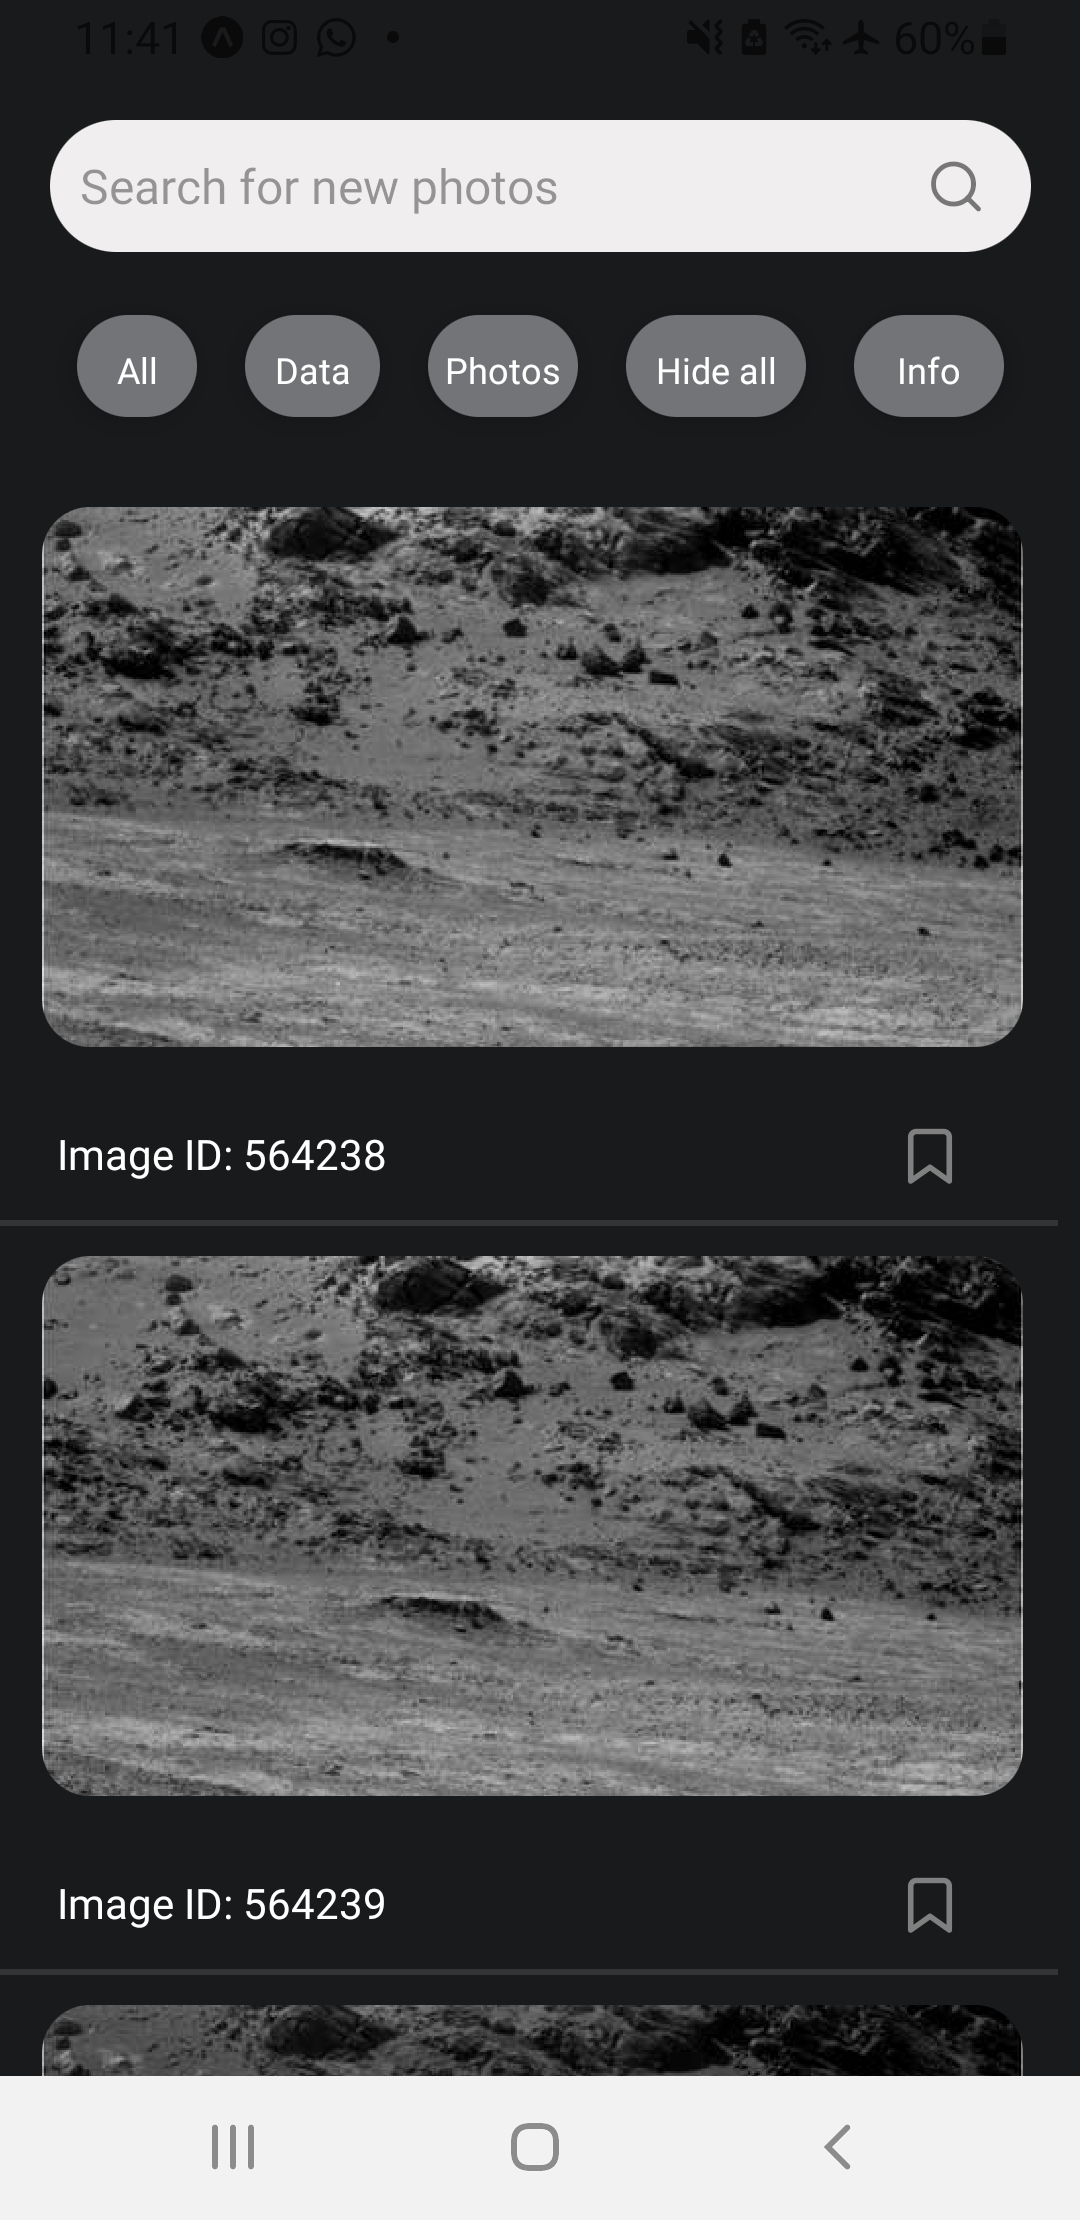
\includegraphics[width=5cm, height=10cm]{images/immaginiAndroid/IndexScreen.jpg}
        \caption{\label{IndexScreenAndroid}Android Index Screen}
    \end{minipage}
    \hfill
    \begin{minipage}[h]{0.47\textwidth}
        \centering
        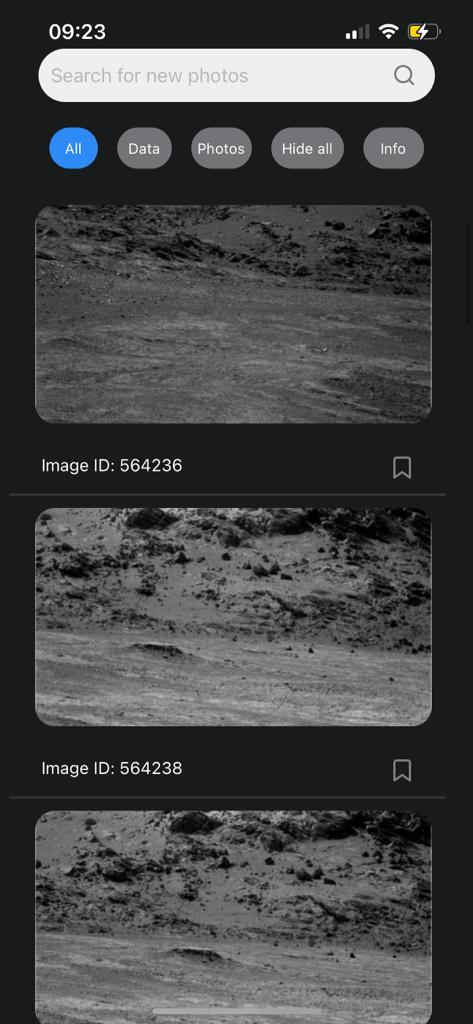
\includegraphics[width=5cm, height=10cm]{images/immaginiPhone/IndexScreen.jpeg}
        \caption{\label{IndexScreenAndroid}Iphone Index Screen}
    \end{minipage}
\end{figure}
\end{document}
